\documentclass{article}

\begin{document}

\setlength{\parindent}{6ex}

\indent

Object detection is a concept of computer vision in which trained models 
detects objects with their category and location in given images or videos. 
As you can see in the figure \ref{fig:dog1}, object detection is both 
classifying and localizing the object instances in given images.

\begin{figure}
    \centering
    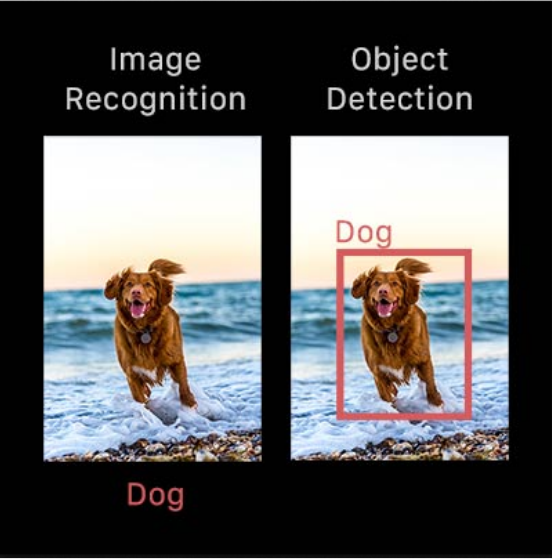
\includegraphics[width=0.5\textwidth]{dog}
    \caption{Difference between recognition and detection}
    \label{fig:dog1}
\end{figure}
\end{document}